\documentclass[twocolumn,10pt,a4j]{jsarticle}
\usepackage{kougai}
\usepackage{dcolumn}


\title{OffscreenCanvasを用いたシミュレータ教材の軽量化}
\author{1532040 岡本 悠祐  指導教員 須田 宇宙 准教授}
\date{}
 
\begin{document}
\maketitle
\section{背景}
シミュレータ教材は不可視現象を可視化する教材である.そのため,イメージが困難な事象への理解促進を促す手法として有用である.
e-Learningの普及に伴いシミュレータ教材の活躍の場が増加し,様々な分野に対応したシミュレータ教材と効率的な開発手法が必要とされている.

磁場や音場などの波形を可視化するシミュレータにおいてFTDT法が広く用いられているが演算回数が多いことから処理速度は決して速くない.

本研究室では昨年,FTDT法を用いたシミュレータ教材にGPUを適用し処理速度を比較する研究を行った.その結果,大幅な処理速度向上が得られたが,ソースコードの変更箇所が多く,
複雑なため容易に実装できないという問題点が浮上した.

その問題点はJavaScriptをマルチスレッド化,描画を行うOffscreenCanvasを利用することで緩和されると考える.

本研究ではOffscreenCanvasを利用したFTDT法を用いたシミュレータ教材の制作を行い,生産性と処理速度を昨年制作したシミュレータ教材と比較することで,有用性の検証を行うことを目的とする.

\section{WebWorkerとOffscreenCanvas}
\subsection{WebWorker}
WebWorkerはJavaScriptでマルチスレッド処理を可能にするAPIである.Workerを利用するには処理ごとにWorkerを分け,
実行するにはサーバーを利用する必要がある.
また,Worker上で描画を行うことができないため描画処理を行いたい場合は,Workerを定義するメインのスレッドに対して描画処理を渡す必要がある.

\subsection{OffscreenCanvas}
OffscreenCanvasはWebWorkerを利用してWorker上で描画処理を可能にするAPIである.

基本ルールはWebWorkerと同様,サーバーを建てる必要がある.
事前にCanvasタグをHTMLないしJavaScriptで生成し,Warkerに処理を譲渡,描画まで行うため,Workerより必要な処理が少なく手軽に実装できる.

\section{検証方法}
平成29年度本学卒業論文である「GPU利用によるシミュレータ教材の演算速度」を拡張し昨年のシミュレータと演算速度を比較,変更箇所を比較することでOffscreenCanvasの実用性の検証を行う.
 
1つのキャンバスを左右に分割することで処理,描画の負荷を分散させ,1,000回計算するごとに時間を計測し,それを10,000回まで行った.
計測では研究室で使用しているMacを用いた.また,OffscreenCanvasの基であるWorkerの処理速度も計測した.
\subsection{制作したシミュレータ教材}
図\ref{fig:one}は複数の音源からから発生する音場を可視化したシミュレータ教材である.

\begin{figure}[h]
 \begin{center}
  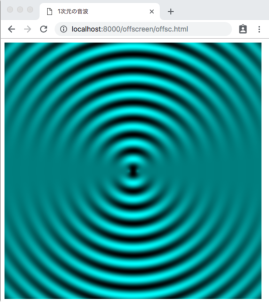
\includegraphics[width=30mm]{sim.pdf}
 \end{center}
 \caption{制作したシミュレータ}
 \label{fig:one}
\end{figure}

\section{検証結果}
CPUを基準とした処理速度を式\ref{eq:eq1}に当てはめて求めた.

キャンバスを分割したWebWorkerとOffscreenCanvasは処理速度が遅い方を参照する.その結果は表\ref{tab:tab1}である.
\begin{equation}
\frac { 各手法10,000回の処理速度 } { CPU10,000回の処理速度 } = 処理効率
\label{eq:eq1}
\end{equation}


\begin{table} [h]
\centering
\caption{各種法の処理速度比較}
	\begin{tabular} {| c | l D{.}{.}{8} |} \hline
	GPU & 1: & 0.810988 \\ \hline
	OffscreenCanvas & 1: & 0.80789763 \\ \hline
	WebWorker & 1: & 62.52562982 \\ \hline
	\end{tabular} 
	\label{tab:tab1}
\end{table}

OffscreenCnavasの変更箇所は分割したキャンバスの範囲指定と,キャンバスの生成元であるHTMLのキャンバスを増やすだけで,ソースコードを変更することはほとんどなかった.
GPUの処理速度と遜色ない処理速度を実現できたため,OffscreenCanvasを用いたシミュレータ教材はFTDT法において有用であるといえるのではないのだろうか.

\section{終わりに}
本研究ではOffscreenCanvasのFTDT法を用いた音場シミュレータへの有用性を検証した.Workerの処理速度の低さと,GPUの処理速度と遜色ない結果が得られたのは正直以外だった.
しかし,実装するだけであれば容易だが,シミュレータとして成立させるため,リアルタイムで数値を変更する場合は,追加箇所が多くなった.
したがって,今後は追加箇所の知識の共有が必要になるだろう.

\begin{thebibliography}{99}

	\bibitem{book}川勝 研太郎:``オフスクリーンキャンバスを使ったJSのマルチスレッド描画 \UTF{2013} スムーズなユーザー操作実現の切り札'',\url{https://ics.media/entry/19043},2018/12/23参照

\end{thebibliography}
\end{document}
